\section{Dataset}
We obtain a large-scale timestamp-aligned dataset of \texttt{<word, subwords, location, activity>}. We present the details of our dataset and quality of it in the following part. 

\subsection{Statistics of the dataset}
\label{sec:dataset}
%\KZ{Because one of the contributions of this paper is the dataset,
	%you should give the stats of the raw videos, number of words segmented out,
	%and then the distributions of the word types, activities and locations, etc.
	%Give a table here.}
The dataset contains 10,779 quadruplets from corresponding 3,068 videos and 5,834 sentences, including 6 different types of dog sounds, 11 location categories, 14 activity categories, and 20 IPA vowels for subwords as shown in ~\tabref{tab:dataset}. We follow the definitions of dog vocalization types defined in Audioset and we adopt the most frequent locations and activities tailored for Shiba Inu by combining commonsense and data manual checking for location and activity. More details of the dataset can be seen in Appendix C. 
%\MY{if you have space, add a textual expalaination to different word types, i.e. howl is a constant high-pitched vocal sound, bow-wow is ....}
%\AT{no more space}
%\MY{appendix abc?}.
%\MY{we follow the definitions of dog vocalization types defined in Audioset} 
%\MY{This sounds amateur, try saying that we listed out the most frequent scenes and activities tailored for Shiba Inu by combining commonsense and data manual checking. e.g. u get information from the subtitles, raw results of pretrained model etc.}. 
%\MY{how? if this sentence is talking about 4.2, then leave everything there}.
%The average, max, min length of a word is respectively 0.8 seconds, 3 and 0.08 seconds. We have averagely 1.7 words in a sentence and 1.5 sentences in a video.  
%\KZ{The filering should have been talked about in approach.}

%\KZ{I think there should be at least one example pic for each of the location/
%activity, to be included in the appendix.}

\begin{table}[th]
	\small
	\begin{tabular}{p{0.15\columnwidth}|p{0.7\columnwidth}}
		\toprule
		\textbf{Context} & \textbf{Possible values} \\ \midrule
		Word Type & Bow-wow, Bark, Whimper, Growl, Howl, Yip \\ \midrule
		Phonetic Symbol & \textipa{\textbackslash u,æ,\textrevepsilon,\textbaru,\textturnm,\textturna,a,\textbaro,\textscoelig,\textschwa,\textupsilon,\textsci,\textturnscripta ,\textepsilon,\textturnv,\textscripta,œ,\textopeno,\textbari,e\textbackslash} \\ \midrule
		Location & Living Room, Food Nearby, Grass, Cage, Road, Bathroom, Snowfield, Beach, Square, Vehical Cabin, Others    \\ \midrule
		Activity & Mount Or Hump (beg), Play With People, Sit, Lay Down, Walk, Sniff, Eat, Stand, Take a Shower, NoDog, Run, Be Touched,  Unknown, Fight With Dogs, Show Teeth or Bit\\ 
		\bottomrule
	\end{tabular}
	\caption{Respective categories for dog vocalizations and contextual information in our dataset.} 
%\KZ{what exactly
%is the definition of ``subword''? Are these syllables or IPA symbols?
%A subword should be a sequence of IPA symbols or a sequence of syllables?}}
	%\KZ{Change ``growling'' to growl everywhere incl.
		%the figures to be consistent, since yip, growl, howl, etc. are both verbs and nouns.}}
%\KZ{How did we define the domains of these values?
	%Please give citations and sources.}}
	\label{tab:dataset}
\end{table}

~\figref{fig:distri} shows the prior distribution of the items in the dataset across different word types, subword IPA symbols, location types, and activity types. This data imbalance reflects real-world data distribution, that pet dogs kept at home are more prone to stay in the living room and exhibit activities like standing and fighting with dogs. We consider this imbalanced prior distribution when computing the correlations between them. 
%\MY{consider saying: this data imbalance reflects real-world data distribution, that pet dogs kept at home are more prone to stay in living room and exhibit activities like laying down and playing with human}. 
%\MY{awkward sentence, just say that we take this imbalanced prior distribution into consideration when computing the correlations between them}.
%\KZ{Add a figure/table to show the stats of the words/sentences that we got,
%like the avg len, min/max len, variance, how many words per sentence, how many
%words per video, etc. These will be interesting stats to show the scale and
%significance of our dataset.}


%\begin{table}[th]
%	\small
%	\centering
%	\begin{tabular}{p{0.2\columnwidth}|p{0.15\columnwidth}|p{0.15\columnwidth}|p{0.15\columnwidth}}
%		\toprule
%		& Min len & Max len & Avg. len \\ \midrule
%		Bow-wow & 0.16s & 2.88s & 0.51s  \\ \midrule
%		Yip & 0.16s & 2.92s & 0.60s\\ \midrule
%		Whimper & 0.16s & 2.76s & 0.62s\\ \midrule
%		Bark & 0.20s & 2.88s& 0.67s \\ \midrule
%		Growl & 0.20s & 2.96s & 0.79s\\ \midrule
%		Howl & 0.16s & 2.96s & 0.98s\\
%		\bottomrule
%	\end{tabular}
%	\caption{Statistics of dataset. The columns are respectively the minimum, maximum and average length of a word.}
%	\label{tab:datainformation1}
%\end{table}

\begin{figure*}[h]
\centering
%\subfigure[Word type distribution]{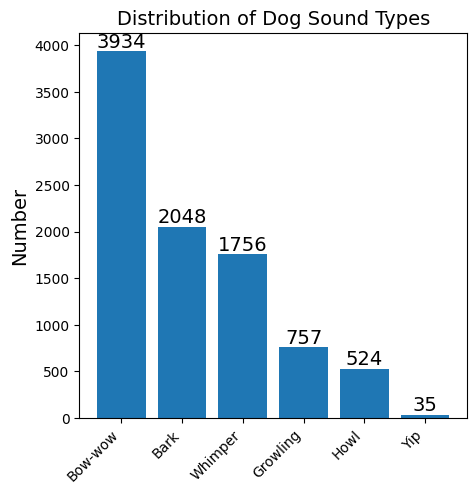
\includegraphics[width=0.32\hsize, height=0.28\hsize]{images/sound_distri.png}}
%\subfigure[Location type distribution]{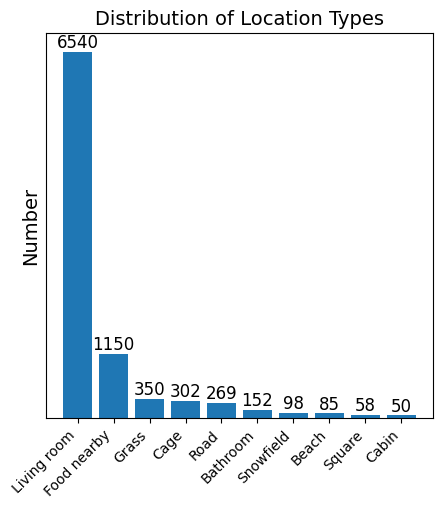
\includegraphics[width=0.32\hsize, height=0.28\hsize]{images/location_distri.png}}
%\subfigure[Activity type distribution]{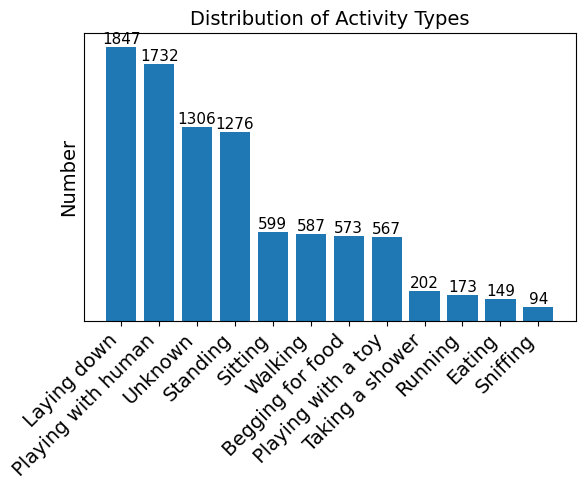
\includegraphics[width=0.32\hsize, height=0.28\hsize]{images/activity_distri.png}}
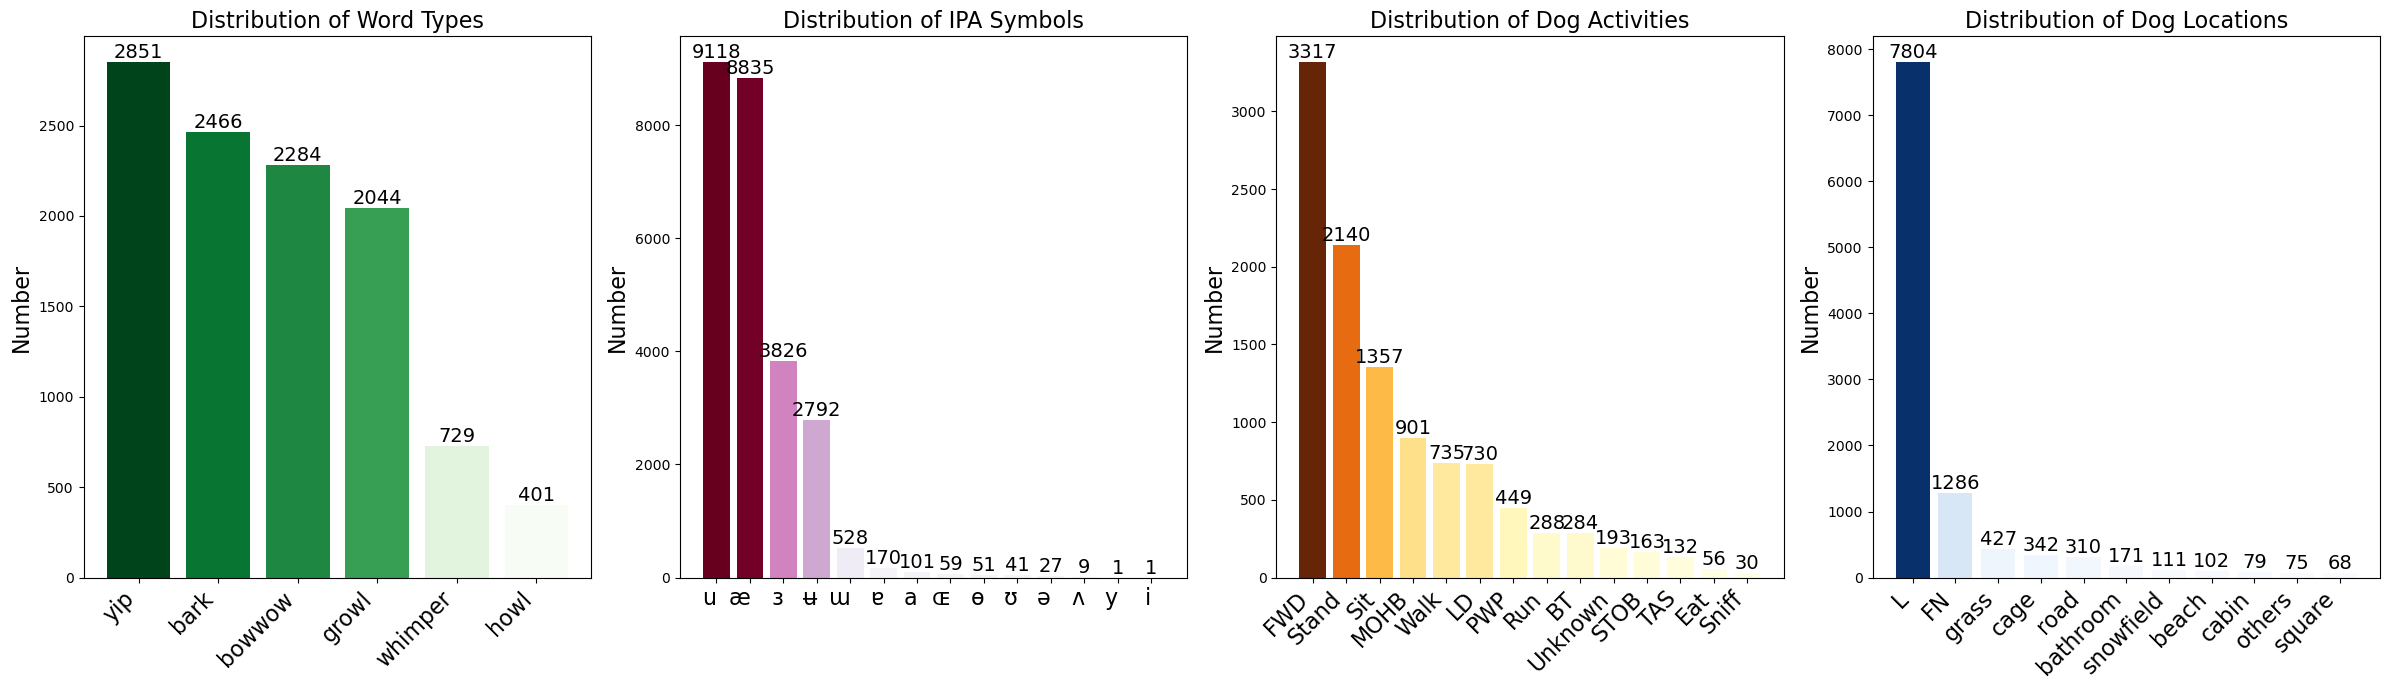
\includegraphics[width=1.8\columnwidth]{images/data_distri.png}
\caption{Prior distributions of word types(green), IPA symbols(pink), locations(blue) and activities(red) in
the quadruplet sequences. The numbers shown are the number of times for different word types, locations, and activities.
``L'', ``FN'', ``FWD'', ``MOHB'', ``LD'', ``PWP'', ``BT'', ``STOB'', ``TAS'' represent  ``Livingroom'', ``Food Nearby'', ``Fight With Dogs'', ``Mount Or Hump (Beg)'', ``LayDown'', ``Play With People'', Be Touched'', ``Show Teeth Or Bit'', ``Take A Shower'' respectively. 
}
%\KZ{These graphs can be flattened to make some space.}} 
%\KZ{Change growling to growl.}} %\KZ{Make these three plots equal size.} \AT{will be modified after having whimper yip result}} 
%\KZ{Always
%add full stop at the end of each caption. Pls make the words on the x-axis slanted a bit (just like (a) to save space. Pls do that for the rest of the figs.
%Why is the Yip so little? In my experience, I hear this kind of sound quite 
%often in the dogs. The distribution is too skewed. Is it possible
%that the recall of Yip is not good enough? Can we present a confusion
%matrix among these 6 types from the classification results?}}
\label{fig:distri}
\end{figure*}

\subsection{Quality of the dataset}
%\KZ{Give the acc numbers of each steps in \figref{fig:method}.}
%\KZ{You need to give details on how you acheive these accuracy numbers.
%Like how u sampled, how many judges, how to judge, etc.}
We present the accuracy of each step to ensure the high quality of our dataset. For word segmentation and word classification, we randomly sample 200 segmented words to listen to. Three annotators have to label whether this is a singular dog word and whether the word is correctly classified. Their respective accuracy is 0.95 and 0.84. We achieve an accuracy of 0.78 for location classification on our manually labeled pictures and an accuracy of 0.59 for the top 1 and 0.9416 for the top 5 for activity classification.

\section{Results and Analysis}
\label{sec:results}
%\KZ{Rephrase this para:
%\MY{rewrite this para, combine with the research questions you raised}
To answer the first question, we analyze the relationship between words and context. We then explore the relationship between words and subwords. We present a summarization of findings that uncovers dog vocalization patterns. To answer the second question, we adopt conditioned probability. 
%In this section, we present our analysis of the data. We analyze the relationship between words and context. We then explore the relationship between words and subwords. We present a summarization of findings that uncovers dog vocalization patterns.
 
\subsection{Correlation between word type and location}
The vocalization of a dog varies depending on its location. Based on the dataset, we compute the correlation between location and word as shown in ~\figref{fig:sound_location}: 
\begin{equation}
\frac{P (\text{location}| \text{word})}{P(\text{location})}
\end{equation}
By dividing each item in the formula by its prior probability, we can offset the influence of the original umbalanced frequencies of the word types and locations. 
%We compute a frequency table of word types and locations, involing counting the occurrences of each unique combination of variables and organizing them into a two-dimensional table. 
%\figref{fig:sound_location} illustrates this relationship.
%\begin{figure}[ht]
%	\centering
%	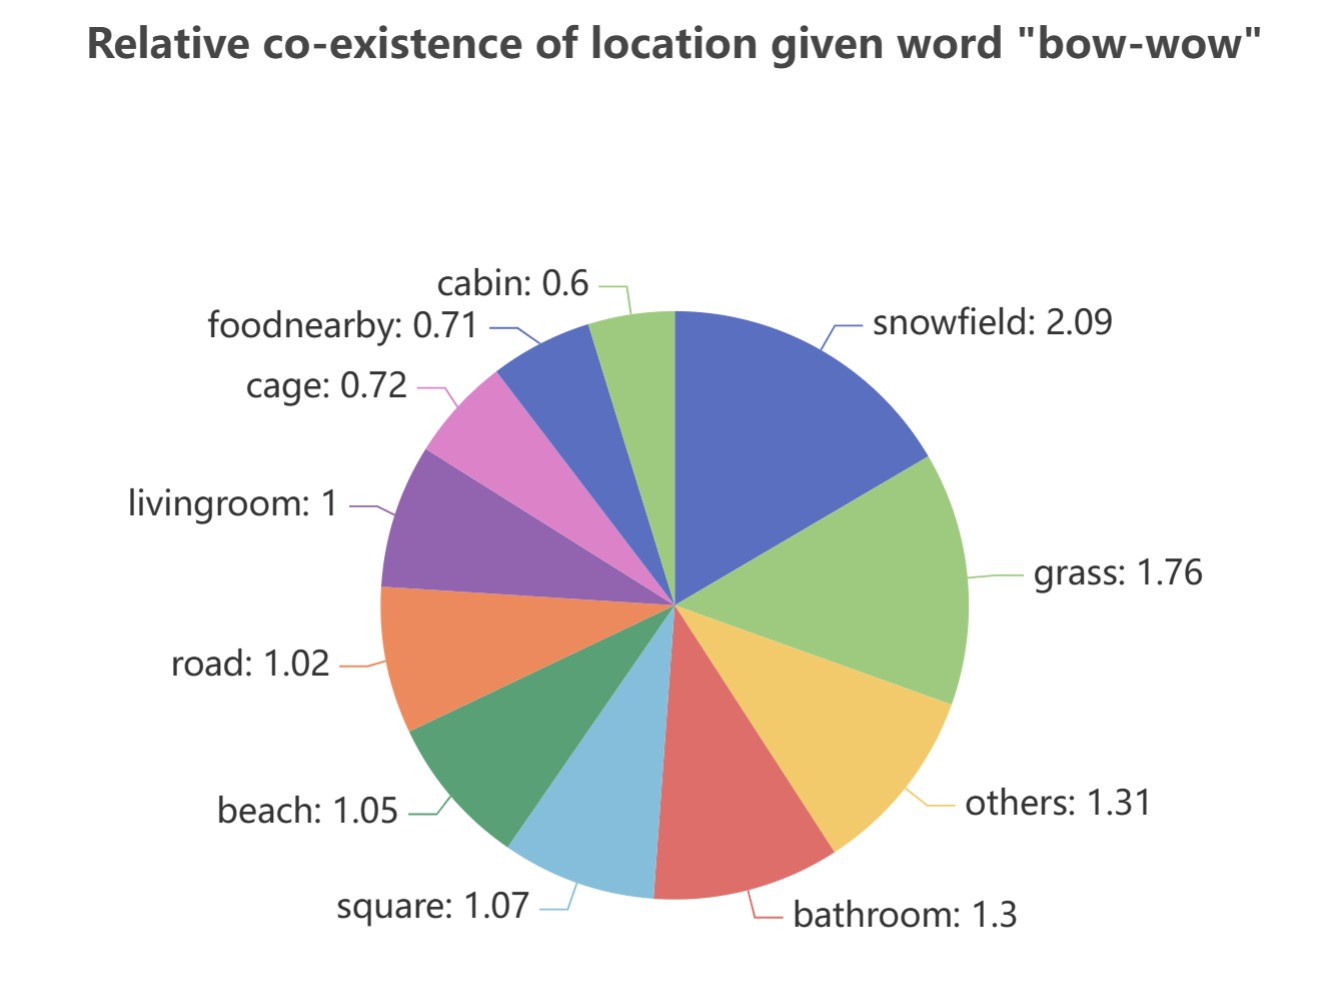
\includegraphics[width=0.8\columnwidth]{images/relative_bowwow.jpg}
%	\caption{
%\KZ{There's actually no such thing called: The relative probability.} 
%The probability of location given word ``bow-wow'' divided by location prior probability.}
%	\label{fig:relative_bowwow}
%\end{figure}

%\MY{For all these results, you should refer to specific numbers/comparisons from the probability, otherwise your readers cannot correspond the interpretations with the results}
%\AT{I explain in each item at which context it tends to do so}

%Our analysis reveals several patterns between dog word types and 
%corresponding locations with a minimum support number of 100 occurrences: 

%\KZ{Replace all uncomfort with discomfort.} 
%\KZ{When you make the following conclusions, what are min supports for each of these observations? 100, 10?}
%\AT{each item presents at least 100 times and each combinations are selected one shown more than 10 times.}
\begin{figure*}[h]
\centering
\begin{subfigure}[]{0.4\textwidth}
	\centering
	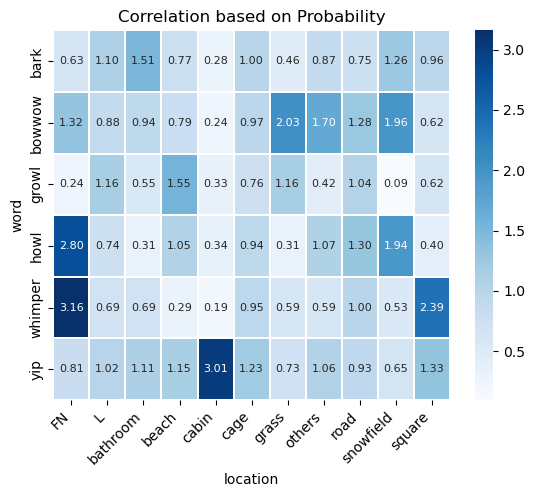
\includegraphics[width=0.86\textwidth]{images/sound_location_prior.png}
	\caption{Correlation between word types and locations.}
%\KZ{If you don't present the formula for each
%of these metrics, we don't even know how you come up with the numbers in
%these matrixes! This is unacceptable!}}
	\label{fig:sound_location}
\end{subfigure}
\begin{subfigure}[]{0.4\textwidth}
	\centering
	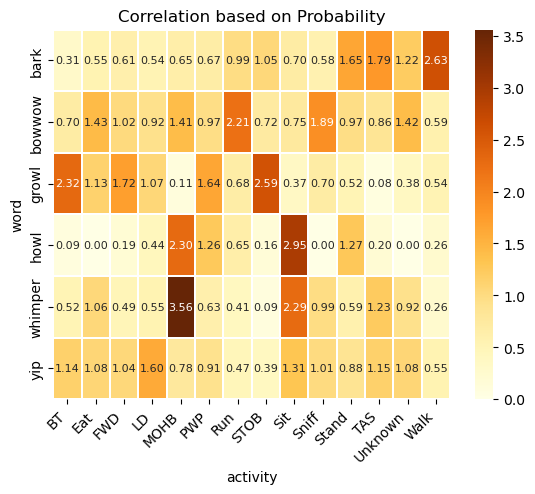
\includegraphics[width=0.86\textwidth]{images/sound_activity_prior.png}
	\caption{Correlation between word types and activities.}
	\label{fig:sound_activity}
\end{subfigure}

\begin{subfigure}[]{0.4\textwidth}
	\centering
	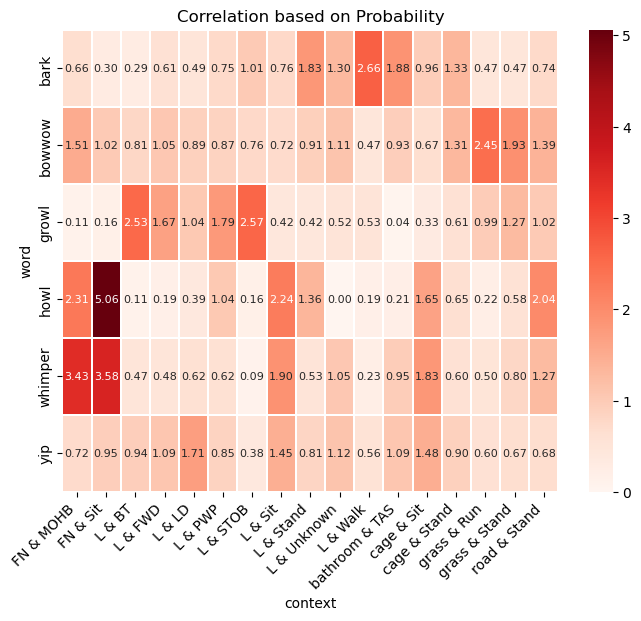
\includegraphics[width=0.86\textwidth]{images/one_sound_context.png}
	\caption{Correlation between word types and contexts.}
\label{fig:one_sound_context}
\end{subfigure}
\begin{subfigure}[]{0.4\textwidth}
	\centering
	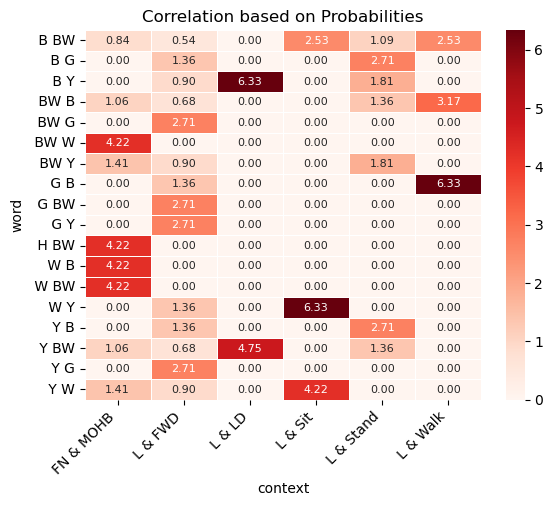
\includegraphics[width=0.86\textwidth]{images/sound_sequence_context.png}
	\caption{Correlation between bi-gram of words and contexts. 
``B'', ``BW'', ``G'', ``H'', ``Y'', ``W'' represent ``bark'', ``bow-wow'', ``growl'', ``howl'', ``yip'' and ``whimper'' respectively.}
	\label{fig:sequenc_sound_context}
%\MY{y axis is sound, make sure that you are consistent in using word/sound to represent processed word types}}
%\KZ{There's both bow-wow growling and growling wow here. And their correlated
%contexts are a bit different. This is interesting. Because when you have AB
%and BA in this table, people might think that they were extracted from a seq
%like ABABA, and this seq should correspond to the same context. But it's not.
%So you should explain.}\AT{Hard to interpret it}}
\end{subfigure}
\caption{Correlation to explore semantics of words.}
\label{fig:correlation}
\end{figure*}

%An example of ``bow-wow'' in snowfields is given in ~\figref{fig:bow-wow_snowfield}.

%\KZ{Do not repeat what is already bolded as headline.}

%\paragraph{``Bark'' can be used to show anger and warning.} Bark, a more abrupt sound compared with ``bow-wow'', conveys many semantics and one of them is to express its anger and warning ~\cite{yeon2007vocal}. When the dog is located in a cage, it tends to ``bark'' as shown in Appendix ~\figref{fig:bark_cage}.
% ``Whimper'' can be used to show discomfort ~\cite{web2018dog} as dog whimpers when it is located in the bathroom when it is likely to take a shower or in a cage.
% as shown in Appendix ~\figref{fig:whimper_attention}, and when in a cabin, it may want to interact with its host. 
\paragraph{``Bow-wow'' can be used to express curiosity.}
Bow-wows are usually used when they are outside and in unfamiliar surroundings like snowfields, grass, and other places. This word may implicate an exploration of the environment. 
\paragraph{``Whimper'' can be seen as attention-seeking when food nearby.}
``Whimper'' can be used to elicit people attention ~\cite{handelman2012canine}. When there is food nearby, they may beg for food. 


\subsection{Correlation between word type and activity}
We use the same method to analyze the relationship between word types and 
activities in \figref{fig:sound_activity} as: 
\begin{equation}
\frac{P (\text{activity}| \text{word})}{P(\text{activity})}
\end{equation}
\paragraph{``Bow-wow'' may indicate movements or food.} Dogs exhibit a preference for using the ``bow-wow'' sound when engaging in activities that involve movement, such as walking and sniffing. ``Bow-wow'' may also be a signal for food as begging for food or eating. 
\paragraph{``Growl'' expresses interation with outside.}
``Growl'' appears to be used to express interactions ~\cite{handelman2012canine}. It is prevalent when be touched, fight with dogs, play with people and show teeth or bite. 
\paragraph{``Whimper'' and ``howl'' are used when relatively steady.}
Dogs are usually howling when sitting down and standing. We find that Shiba Inu tends to ``howl'' when they are begging for food which is a new observation. 
Dogs often ``whimper'' when engaged in activities like sitting and begging for food. It may indicate contact seeking and a kind of submission ~\cite{pongracz2010barking}. 


%\MY{how is this different from 5.1 section where you say whimper is attention for food}
%\AT{because different words can also express the same meaning}
%\KZ{$P(act | word)$}
%An example of ``bow-wow'' in movements is given in ~\figref{fig:bow-wow_walking}.
%\MY{is this steady? your para title says howls is steady. now there are 3 different words for food, weird...}. 
%\AT{these two sounds needs to be relatively unmoved to express}

\subsection{Correlation between word type and context}
When putting location and activity together as in ~\figref{fig:one_sound_context}:
\begin{equation}
\frac{P (\text{(location, activity)}| \text{word})}{P(\text{(location, activity)})}
\end{equation}
Because of the numerous combination possibilities for context, we define a threshold value of 100, indicating that a particular combination is considered statistically significant only if it occurs more than 100 times. ~\figref{fig:one_sound_context} depicts this relationship between word type and context.
\paragraph{``Howl'' and ``whimper'' come up frequently with food.} ``Whimper''represent attention-seeking, thus it can be interpreted as attention for food when ``food nearby'' and the dog ``begs''. ``Howl'' is used when sitting and food nearby. 
\paragraph{``Yip'' and ``whimper'' can express discomfort.}  They can express pain or discomfort ~\cite{yeon2007vocal,web2018yip}. When the dog is located in the cage and laying down, it tends to yip and whimper.  
\paragraph{``Bark'' can express discomfort.} Shiba Inu barks when it is taking a shower in the bathroom. This can express its discomfort and warning ~\cite{yeon2007vocal} because dogs usually don't like baths. 

%\KZ{\[P((loc, act) | word)\]}
%\KZ{Rephrase: we set a threshold number to be 100, which means if and only this combination occurs more than 100 times then we think this 
%is statistically important.} 
%An example is given in ~\figref{fig:yip_cage}.
%\MY{how is shower indicative of anger? this is very bold argument}
%\item When the dog is located in the cage, as the cage is small, it has to sit down and it may feel anger and ``bark''. 
%\item ``Howl'' and ``whimper'' can be seen as a signal for food. We think these two sounds express imploration and begging.


\subsection{Analysis of the sequence of quadruplets} 
To analyze quadruplet sequences, we start by picking words in the same sentence where the word type changes. We hypothesize that a sequence of different word types in a similar context carries a specific meaning. We only consider combinations that appear frequently, setting a threshold of 10 to distinguish patterns from chance occurrences. We explore the formula as shown in ~\figref{fig:sequenc_sound_context}:
\begin{equation}
\frac{P (\text{(location, activity)}| (w_1;w_2))}{P(\text{(location, activity)})}
\end{equation}
while $(w_1;w_2)$ represents two consecutive words with different types, which is defined as a \textit{bi-gram} here. We highlight several insights. Our findings suggest that the sequence of words might not strongly indicate distinct semantic meanings. For instance, comparing "Bark Bow-wow" and "Bow-wow Bark" reveals differing context distributions. However, in the cases of "Whimper Bow-wow" and "Bow-wow Whimper", we observe similar distributions despite the word order variation.
%\MY{this section is verbose, please read through and make it clear and concise}
%\KZ{\[P ((loc, act) | (w_1; w_2)) \]}

%We find that the sequence of the words may not be very indictive of different semantic meanings. For example, ``Bark Bow-wow'' presents a different context distribution compared with ``Bow-wow Bark''. But ``Whimper Bow-wow'' and ``Bow-wow Whimper'' show the similar distribution. 
%\item Normally, a combination of ``BA'' may have a similar distribution of probability of ``AB'', as they all may come from a sequence like ``ABABA''. But here, our data distribution of ours is unlike this. It may be because the order of the sounds is also part of its semantics. 

%\subsection{Analysis of bi-gram probability}
%To facilitate the comprehension, we further divide each item by $w_2$ 
%prior distribution to show relative changes. 
To provide additional evidence, we examine the bi-gram probability of two-word sequences as $w_1$ followed by $w_2$, where $w_1$ and $w_2$ represent two words. To enhance clarity, we normalize each item by dividing it by the prior distribution of $w_2$, revealing relative changes. The result for: 
\begin{equation}
{P (w_1|w_2)}
\end{equation}
is shown in ~\figref{fig:w2w1}. As observed, ``howl'' and ``whimper'' are highly probable of following each other and this implies their semantics are kind of overlapping. Same for ``bark'' and ``bow-wow''. This shows the words contain multiple semantics.
\begin{figure}[t]
\centering
\begin{subfigure}[]{0.4\textwidth}
	\centering
	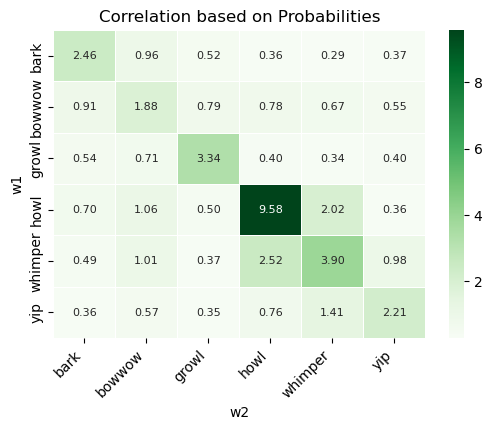
\includegraphics[width=0.85\textwidth]{images/w2w1.png}
	\caption{Correlation based on probability for P($w_2$|$w_1$).}
%\MY{for this fig, font size of each category can be enlarged, i.e. bark bow-wow etc., while the whole figure can be smaller}}
	\label{fig:w2w1}
\end{subfigure}
\begin{subfigure}[]{0.4\textwidth}
	\centering
	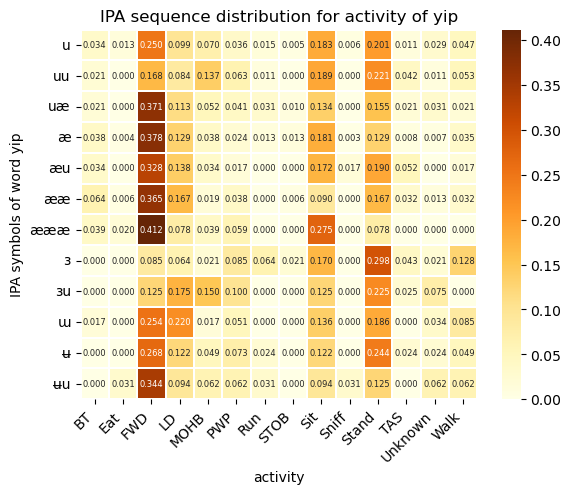
\includegraphics[width=0.9\textwidth]{images/ipa_yip.png}
	\caption{Activity distribution of most frequent subword combinations for yip.}
	\label{fig:subwords_yip}
\end{subfigure}
\caption{Exploring sequence of words and activity distribution of subwords for yip}
%\KZ{There should be a caption for the whole fig here.}}
\end{figure}



%\KZ{I think something can be said such as:
%BW often follows B, but B doesn't follow BW as much. BW also follows G, but
%no so much after H, many words can follow W, and after a Y, there's always a
%BW. Some of the these bigrams we have meanings, others we don't. But at least
%we know these are the popular patterns for future study?}
%\AT{This is because we do not divide them by prior probability, which is asked not to do so.}

%\KZ{I think something can be said such as:
%BW often follows B, but B doesn't follow BW as much. BW also follows G, but
%no so much after H, many words can follow W, and after a Y, there's always a
%BW. Some of the these bigrams we have meanings, others we don't. But at least
%we know these are the popular patterns for future study?}
%\AT{This is because we do not divide them by prior probability so we have such feeling, which is asked not to do so. }

\subsection{Analysis of subwords semantics}
Previous works show for one word type, it conveys multiple meanings. Each word contains one or multiple different subwords. By combining analyzing the multiple meanings for one word type and its possible subwords, we prove that one word type can be further divided into finer-grained types, which is the first data-driven experimental proof. For subwords in the same word, we first collect the most frequent subwords that can be one or a sequence of IPA vowel symbols, then we illustrate their distribution on the context and they vary a lot, which means that they convey different semantics. As shown in ~\figref{fig:subwords_yip}, we present the activity distribution of the most frequent subwords for yip. As we can see, for the same scene fight with dogs, different IPA symbol sequence shows an dissimilar distribution. 

We further observe that these frequently different subwords are not restricted to one dog, which means this semantic difference is not by accident or caused by specific characters of one dog. A summary table is appended in Appendix C. By combining analysis of words and subwords, we explore that the distribution of the IPA symbol is mainly influenced by the distribution of the word which contains this symbol and this illustrates that the minimal semantic unit is word-related instead of subword. A detailed explanation is in Appendix D.
%\MY{this sentence is confusing, don't know what you mean}.
%\MY{give detailed appendix sections, e.g. Appendix B. section}. 
%\MY{avoid using prove, it is a strong claim, just say find/observe} 
%\MY{same here}. 
%For sequence of same subwords shown in one word, we assume this sequence of same ipa symbol can be replaced by a longer IPA vowel. For example, a sequence of ``u'' vowel can be replaced by ``u:''. We find the influence of consistent repeating subwords on semantics are subtle. The details of explanation is in Appendix. 

%1. each words may contains different transcript, different subwords. 
%2. this is because each word type contains multiple meanings. 
%3. For same word, same transcripts are from different dogs. 
%4. In same context, for same ipa pattern for specific word, these patterns are from different dogs. 

\begin{table}[t]
\small
\centering
\begin{tabular}{p{0.13\columnwidth}|p{0.45\columnwidth}|p{0.3\columnwidth}}
\toprule
\textbf{Lexical Symbols} & \textbf{Previous Meaning} & \textbf{Our Meaning}\\
\hline
Whimper & attention-seeking \cite{handelman2012canine},
				discomfort \cite{web2018dog} & attention-seeking, beg for food, steady, discomfort \\
\hline
Yip & discomfort ~\cite{web2018yip} & loneliness \\
\hline
Bow-wow & NA & show curiosity, movement\\
\hline
Growl & playing interaction ~\cite{handelman2012canine} & interation with outside \\
\hline
Bark & warning \cite{handelman2012canine} & discomfort \\
\hline
Howl & warning, play, group cohesion ~\cite{ani8080131} & signal for food, steady \\
%\hline
%Bark Bow-wow & NA & discomfort \\
%\hline
%Bow-wow Howl & NA & signal for food \\
%\hline
%Whimper Bow-wow & NA & signal for food \\
\bottomrule
\end{tabular}
\caption{Summary of findings with comparison to previously-discovered meanings.}
%\KZ{The first column of this table has too much white space.
%I think this table might be narrowed down to one column. We need to make some
%space for more detailed analysis and discussions.}}
%\KZ{Caption is either on the top
%or on the bottom. Be consistent. Make this table a narrow one. Use
%acronyms to save space.}}
\label{tab:finding}
\end{table}




\subsection{Comparison with Previous Works}
%\KZ{At the end of this, we can have a table that summarizes all the 
%interesting findings: word/bigram, the meaning we discovered, its previously
%known meaning, citation of prev meanings.}
We present our findings including the evidence to support previous theoretical studies and our new observations in \tabref{tab:finding}.
Through the analysis, we found most of the patterns we mentioned are consistent with the previous qualitative research. We also discover more detailed interpretations of those existing patterns and provide possible new findings. We are the first web-data-driven approach to analyze the minimal semantic unit of the Shiba Inu dog language.  

%\MY{u discover more detailed interpretations of those existing patterns, and provide possible new findings. then give examples, possibly using the bi-gram results as previously no one does this }
%\AT{if doing so, it may be redundant as i explained in each item which words have new meaning and which are consistent with existing research}


%``Bow-wow'' can be seen as a low-pitch ``bark'' and previous work like conflating them. Our findings suggest ``bow-wow'' and ``bark'' have a lot in common, but ``bow-wow'' has its own unique meaning, dissimilar to ``bark''. 



%\begin{table}[th]
%\small
%\begin{tabular}{p{0.2\columnwidth}|p{0.7\columnwidth}}

%\toprule
%\textbf{Findings} & \textbf{Explanation} \\ \midrule
%Conformity & 
%\makecell[l]{1.``Bark'' can show the anger and warning. \\
%2.``Growl'' expresses playing interaction.\\
%3.``Whimper'' can be seen as attention-\\seeking and a sign of discomfort. \\
%4.``Yip'' is a signal of discomfort.}
% \\ \midrule
%New observations & 
%\makecell[l]{
%1.``Bow-wow'' can be used to express \\curiosity and it is usually seen when \\dog is in movement.\\
%2.``Bark Bow-wow'' are highly used when \\dog is forced. \\
%3.``Bow-wow Howl'' and ``Whimper Bow-\\wow'' are usually used for asking food.}
% \\ 
%\bottomrule
%\end{tabular}
%\caption{Overall findings of the analysis.}
%\label{tab:findings}
%\end{table}

%\KZ{Maybe try this to summarize the findings in comparison with the
%previous studies?}
%\AT{new findgins means that we find something that never mentioned before, but we do not show contradictions with previous work}





%People believe:
%\begin{itemize}
%\item Bark: short-range interaction; high pitch are made in isolation situation, stranger; 
%\item Growl: agonistic interactions as a warning or threatening signal or during play interactions. 
%\item whine: indicators of stressful arousal but also greeting and attention-seeking behaviours
%\item howls, which maintain group cohesion
%\item groans and yelps, signs of acute distress and acute pain, respectively; and grunts, which are considered as pleasure-related signals
%\item They mainly use short-distance calls in interactions with humans, like barks, growls, and whines, compared with long distance calls, which are used instead to communicate with conspecifics
%\end{itemize}

%Conformity:
%the difference between bow-wow and bark: mainly frequence

%\begin{itemize}
%\item Whimper sttention-seeking cabin, food, cage
%\item Bark anger, high pitch are made in isolation situation(located in a room isolated from its owner) like in cage
%\item growling: play interaction
%\item howl draw attention for begging for food
%\item bark bow-wow when bathing, discomfort
%\end{itemize}

%Our new finding:
%\begin{itemize}
%\item Bow-wow can be used to show dog exploring the outside world or curiosity;
%\item Growling may also show enjoyment when the dog is laying down and eating;
%\item Dogs like to bow-wow when moving around; and like to howl, whimper, or 
%yip when they are stationary.
%\end{itemize}
